\section{Design}
\label{sec:design}

In the overall design a modular approach has been chosen. This is done to devide the code into logic pieces, each with a clear cut role - much similar to the object oriented style from C++ or Java. Following this pattern makes the code easier to grasp - and to re-use for future use.

%The connections on the network will be set up using sockets in C. The sockets will use TCP as a reliable transfer protocol. This way any message is assumed delievered once sent. 

To keep the system going the messages are passed between the sensor nodes and the user. These messages are showvn in Figure~\ref{fig:messages}.
\begin{figure}[ht!]
\centering
    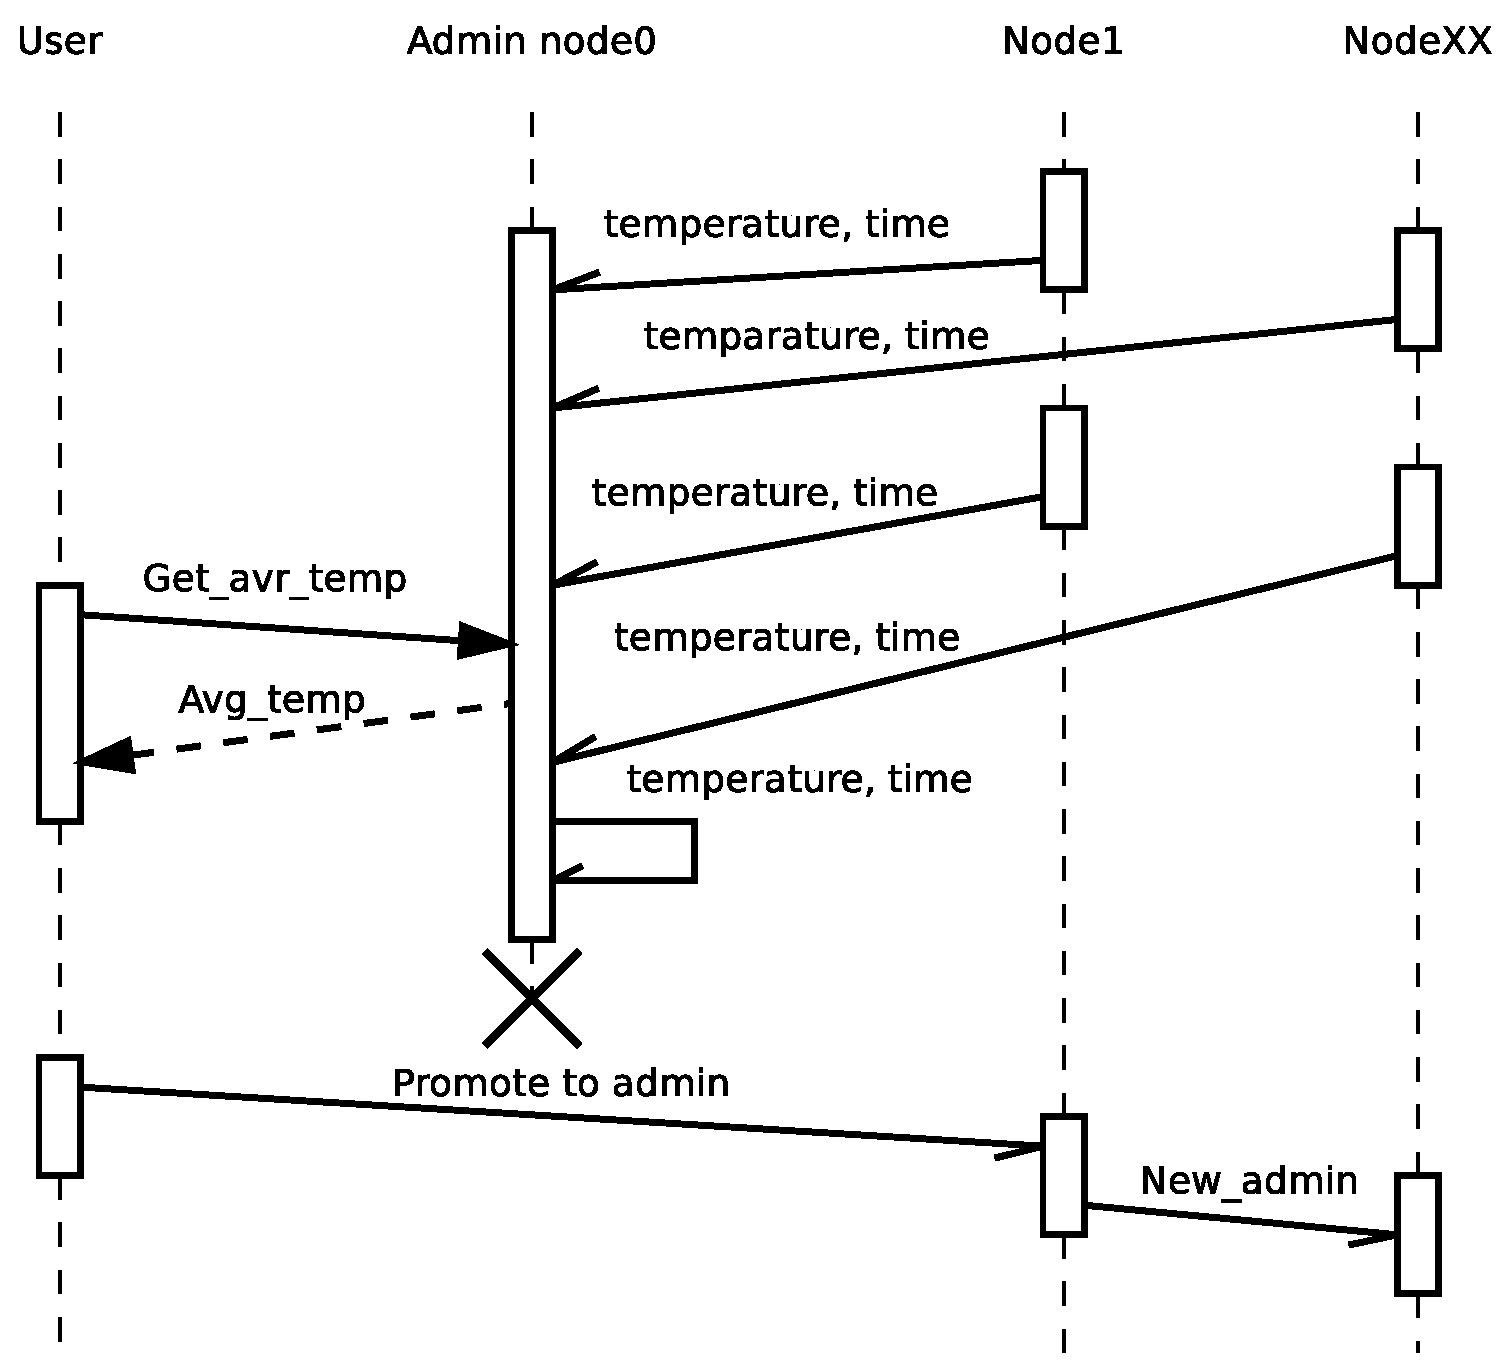
\includegraphics[scale=0.4]{eps/communications2}
\caption{Messages in the system}
\label{fig:messages}
\end{figure}

These messages are sent using \textit{at-most-once} semantics, through TCP. This way the application level software only has to hand over the message to the transport layer and it will be sent reliably.

As it is shown in Figure~\ref{fig:messages} every node has to fill the role as a sensor. That means that the admin node has to have two roles. To achieve this the sensor software is devided into three parts - one for each of the jobs mentioned in section \ref{sec:proposedsolution}. With a clear seperation it is possible for the admin node to send temperature data to itself and thus keep working with two roles.

Special care must be given to the fact that there might be several master nodes operating at the same time. This can happen when first master node goes down and next node is promoted to be a master node. In the case that first master nodes comes up thinking that it is still a master node, there will be a situation with two master nodes working at the same time. To prevent this each promotion to master node from simple node carries a promotion key. The promotion key is increased by the user node each time a new promotion is done. When master node announces itself to be a master node by broadcasting this information, it includes the master key in an announcment. If temperature node receives announcement from a node with a master key lower than current configured, this announcement will be ignored.

%%%%%%%%%%%%%%
%%%% The following might be implementation description ...?
%%%%%%%%%%%%%%
